\scanpage{60}
We then see that
\[
x\prec y\text{ and }y\prec z\quad\Longrightarrow\quad x\prec z
\]
for let $u,v\in\Sigma_{\unsure{<|*}}(1)$ be such that
\[
\mathord{\rlap{$\deleted{\unsure{s}}$}p}_1 u=x,\quad\uline{b}u=\underbrace{y,\quad p_1}v=y,\quad\uline{b}v=z
\]
% In the first glyph the possible cancelled s overlaps the head of p;
% the earlier letter is unresolved. The short brace is spatial: it lies
% beneath the first y toward the following p_1, not beneath both complete equalities.
we thus have
\[
\unsure{\uline{b}}u=p_1v
\]
% This b and its underline are heavily overdrawn. No earlier character is assigned.
thus by the cartesian square of (38), \deleted{$\exists\unsure{w|u}$}
\[
\exists\mid\ d\in\Sigma^{\unsure{<|*}}(2),\quad\text{with}\quad\uline{b'}(d)=v,\quad p_2(d)=u
\]
let
\[
w=\uline{s'}(d)\in\Sigma^{\unsure{<|*}}(1)
\]
we have
\[
\begin{aligned}
p_1(w)&=p_1(\uline{s'}(d))\overset{(38)}{=}p_1p_2(d)=p_1(u)=x\\
\uline{b}(w)&=\uline{b}(\uline{s'}(d))=\uline{b}(\uline{b'}(d))=\uline{b}(v)=z
\end{aligned}
\]
thus
\figure{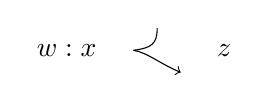
\begin{tikzpicture}[baseline=(x.base)]
\node (x) at (0,0) {$w:x$};
\node at (2,0) {$z$};
\draw (1.15,.28) .. controls (1.15,.08) and (1.08,.03) .. (.85,0);
\draw[->] (.85,0) .. controls (1.03,-.03) and (1.2,-.18) .. (1.45,-.28);
\end{tikzpicture}}.
Moreover, we have
\[
x\not\prec x\qquad\left(\text{for }\operatorname{Im}(\Sigma_1\overset{(p_1;\uline{b})}{\relbar\joinrel\relbar}\Sigma\times\Sigma)\cap\text{diag}=\varnothing\right)
\]
% The final = empty-set and the end of the parenthesis continue below at the right.
thus the relation $x\prec y$ is the relation
of strict inequality associated with an order
relation on $\Sigma$. We recover $\Sigma^{\unsure{<|*}}(1)$ as
the graph of the strict order relation,
$\Sigma^{<}(2)$ as the flags $x\prec y\prec z$ of
length $2$ in \illegible{1} $\Sigma$, and the maps
% A separate small curved upright is raised in the gap after dans, before Sigma;
% its value is unassigned. It is preserved above as an unread fragment.
% Pale lower-left foliation, apparently another hand; no top authorial number is visible.
\margin{59}
